\chapter{Introducción}
El objetivo de este proyecto es construir un software con el que poder visualizar e interactuar con los datos DICOM obtenidos al someter a una escultura a una Tomografía Axial Computerizada (TAC). 

Para ello se hará uso de VTK, que proporciona una serie de librerías en C++ para facilitar operaciones sobre datos DICOM, y de Qt, para la Interfaz Gráfica de Usuario (GUI).

Antes de empezar con el proyecto en sí, se definirán conceptos como DICOM o TAC que se usarán a lo largo de éste y conviene saber lo que son, así como las distintas herramientas que se utilizarán.

\section{DICOM}
DICOM (\textit{Digital Imaging and Comunication in Medicine}) es el estándar internacional para manejar, visualizar, almacenar, imprimir y transmitir imágenes de pruebas médicas (ISO12052) \cite{about_dicom}.

Pese a que su uso está mayoritariamente extendido en el campo de la medicina, se puede usar en otros, como el de la restauración de bienes culturales, como es el caso de este proyecto.

En un archivo DICOM hay almacenado, además de metadatos, una imagen \cite{dicom_classes_vtk} (Figura~\ref{fig:prostate_dicom}).

\begin{figure}[H]
	\centering
	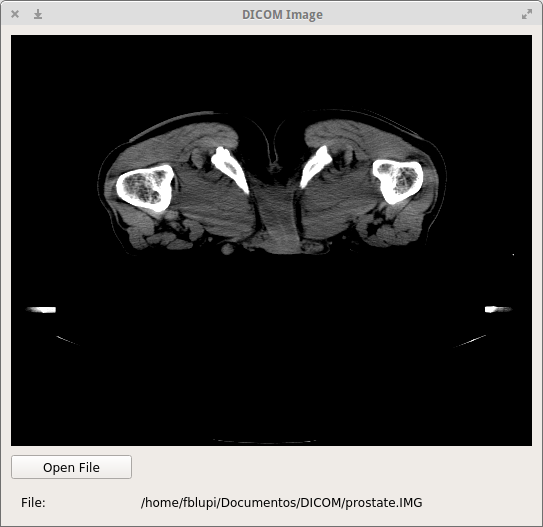
\includegraphics[width=10cm]{imagenes/prostate_dicom}
	\caption{Imagen DICOM de una próstata visualizada con un programa diseñado para visualizar archivos DICOM.}
	\label{fig:prostate_dicom}
\end{figure}

Cuando se realiza un TAC se obtiene una serie de imágenes (Figura~\ref{fig:brain_dicom_serie}) de rebanadas del objeto al que se realiza el escáner. Éstas imágenes son archivos DICOM, y con todas ellas se puede llegar a construir un modelo volumétrico.

\begin{figure}[H]
	\centering
	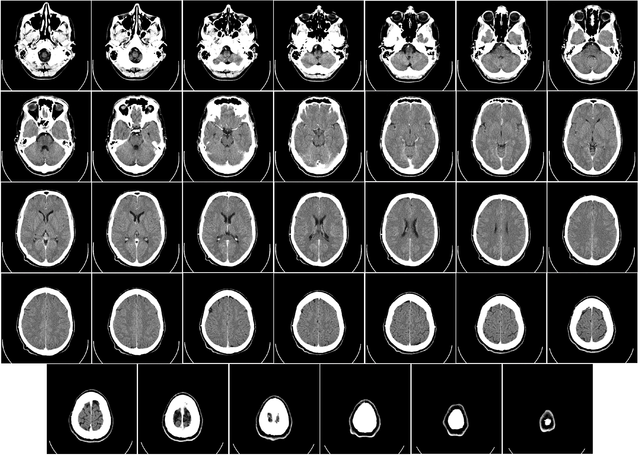
\includegraphics[width=10cm]{imagenes/brain_dicom_serie}
	\caption{Serie de imágenes DICOM extraídas de un TAC realizada a un cerebro.}
	\label{fig:brain_dicom_serie}
\end{figure}